% debut d'un fichier latex standard
\documentclass[a4paper,12pt,twoside]{article}

% Pour les unités SI
\usepackage{siunitx}
% pour l'inclusion de figures en eps,pdf,jpg
\usepackage{graphicx}
% quelques symboles mathematiques en plus
\usepackage{amsmath}
% le tout en langue francaise
%\usepackage[english]{babel}
% on peut ecrire directement les caracteres avec l'accent
% a utiliser sur Linux/Windows
\usepackage[utf8]{inputenc}
\usepackage[T1]{fontenc}

% pour faire des systèmes d'équations
\usepackage{systeme}
\setcounter{tocdepth}{3} % Augmente le niveau affiché dans la table des matières

% a utiliser sur le Mac
%\usepackage[applemac]{inputenc}
% pour l'inclusion de links dans le document
\usepackage[colorlinks,bookmarks=false,linkcolor=blue,urlcolor=blue]{hyperref}
\usepackage{subcaption}
\paperheight=297mm
\paperwidth=210mm

\setlength{\textheight}{235mm}
\setlength{\topmargin}{-1.2cm} % pour centrer la page verticalement
%\setlength{\footskip}{5mm}
\setlength{\textwidth}{15cm}
\setlength{\oddsidemargin}{0.56cm}
\setlength{\evensidemargin}{0.56cm}

\pagestyle{plain}

% quelques abreviations utiles
\def \be {\begin{equation}}
\def \ee {\end{equation}}
\def \dd  {{\rm d}}

\newcommand{\mail}[1]{{\href{mailto:#1}{#1}}}
\newcommand{\ftplink}[1]{{\href{ftp://#1}{#1}}}
%
% latex SqueletteRapport.tex      % compile la source LaTeX
% xdvi SqueletteRapport.dvi &     % visualise le resultat
% dvips -t a4 -o SqueletteRapport.ps SqueletteRapport % produit un PostScript
% ps2pdf SqueletteRapport.ps      % convertit en pdf

% pdflatex SqueletteRapport.pdf    % compile et produit un pdf


% ======= Le document commence ici ======

\begin{document}
% Le titre, l'auteur et la date
\title{Exercise 3: Pendulum with a vertical excitation\\{\small Physique Numérique I}}
\date{\today}
\author{Delphine Martres et Damien Korber\\{\small \mail{delphine.martres@epfl.ch} et \mail{damien.korber@epfl.ch}}}
\maketitle
\tableofcontents % Table des matieres
\newpage % Si la toc est trop grande, voir ligne 19.
% Quelques options pour les espacements entre lignes, l'identation
% des nouveaux paragraphes, et l'espa	cement entre paragraphes
\baselineskip=16pt
\parindent=15pt
\parskip=5pt



%%%% ON COMMENCE A ECRIRE D'ICI

\section{Introduction}

\section{Analytical computations}
%TODO : Revoir en détail cette partie: Y'a eu l'ajout de la boîte entre deux, donc il faut vérifier que tout soit encore d'actualité.
\subsection{Differential equation of the problem}
After some computations described in appendix \ref{ann:eq-diff}, equation \ref{eq:equa-diff} results.%TODO : Faire l'annexe en question.

\begin{equation}
	\ddot{\theta} = -\frac{\kappa}{m}\dot{\theta} - \frac{g}{L}\sin\theta
	\label{eq:equa-diff}
\end{equation}
where $\kappa$ is an air resistance coefficient, $m$ is the mass, $\theta$ is the angle of the pendulum, $g$ the mean gravity on earth and $L$ the length of the rod.

Equation \ref{eq:equa-diff} can also be written as equation \ref{eq:equa-diff-sys}, which is better for numerical computations.

\begin{equation}
	\frac{d}{dt}
	\begin{pmatrix}
		\theta \\ \dot{\theta}
	\end{pmatrix}
	= \begin{pmatrix}
	\dot{\theta} \\
		-\frac{\kappa}{m}\dot{\theta} - \frac{g}{L}\sin\theta
	\end{pmatrix}
	\label{eq:equa-diff-sys}
\end{equation}

\subsection{Mechanical energy and power of non-conservative forces in the frame of reference $R'$}
The only energy to consider is the kinetic energy of rotation, and the potential energy, as there is no translation.
The kinetic energy of rotation is given by $E_{c,r} = \frac{1}{2}I\omega^2$, where $I$ is the moment of inertia and $\omega$ the angular velocity.
The moment of inertia of a solid can be tough to compute for generic objects, but for a discrete number of masses, the moment of inertia is given by equation \ref{eq:moment-inertie}. \cite{ans:moment-inertie} %TODO : Ajouter à la bibliographie le livre de meca pour la formule de I.

\begin{equation}
	I = \sum_\alpha m_\alpha r_\alpha^2
	\label{eq:moment-inertie}
\end{equation}
where $m_\alpha$ is the mass and $r_\alpha$ is the distance between the origin considered and the mass.

In the case of the pendulum, it is quite trivial to compute.
The mass of rod of the pendulum is ignored, and the mass $m$ of the pendulum is condensed in a single point at a distance $L$ of the origin of $R'$.
The moment of inertia is given by $I=mL^2$.\\ %TODO : J'ai pas trouvé de traduction de "point matériel".

The mechanical energy is then expressed as equation \ref{eq:emec}.

\begin{equation}
	E_m = \frac{1}{2}I\omega^2 - mgL\cos\theta =  \frac{mL^2}{2}\dot{\theta}^2 - mgL\cos\theta
	\label{eq:emec}
\end{equation}

Regarding the power, there is only one force to consider, the air resistance (or drag), because it is the only non-conservative one.
The power is expressed as $P = \mathbf{F}\cdot\mathbf{v}$, and the drag is defined as $\mathbf{f} = -\kappa\mathbf{v'}$ in this report, where $\mathbf{v'}$ is the speed in the frame of reference $R'$.
These vectors are given by:

\begin{align*}
	\mathbf{f} =
	\begin{pmatrix}
		f\cos\theta \\
		f\sin\theta \\
		0
	\end{pmatrix}
	= \begin{pmatrix}
		f\cos\theta \\
		f\sin\theta \\
		0
	\end{pmatrix}
	\text{ and }
	\mathbf{v} =
	\begin{pmatrix}
		-v'\cos\theta \\
		-v'\sin\theta \\
		0
	\end{pmatrix}
	= \begin{pmatrix}
		-\dot{\theta}L\cos\theta \\
		-\dot{\theta}L\sin\theta \\
		0
	\end{pmatrix}
\end{align*}

The power of the drag is then given by equation \ref{eq:power}.
\begin{equation}
	P = \kappa\dot{\theta}^2 L^2
	\label{eq:power}
\end{equation}


\subsection{Solutions for little movements around equilibrium}\label{sec:sol-analytique}
%TODO : à remplir
%TODO : Mettre la solution analytique finale avec eq:sol-analytique-gen comme label.
\section{Numerical computations}

\subsection{Little movements without excitation or air resistance}
In this section, no excitation or air resistance will be considered: $\kappa = 0$, $d = 0$.
The movements are small, and approximations are made: $\theta_0 = \num{d-6}$, $\dot{\theta}_0 = 0$.
The computations run for \SI{20}{\second}.

\subsubsection{Comparison between the analytical solution and the approximation of Stormer-Verlet method}
The problem is easy enough to be able to compute the analytical solution.
The general solution was given in section \ref{sec:sol-analytique} by equation \ref{eq:sol-analytique-gen}.
Using the defined initial conditions, the constants can be computed, and the analytical solution for this problem is given by equation \ref{eq:a-sol-ana}.

\begin{equation}
	\theta = 10^{-6}\cos(\omega_0t)
	\label{eq:a-sol-ana}
\end{equation}

It is then possible to compare the analytical solution with the solution found using the numerical method of Stormer-Verlet, which is done in figure \ref{fig:a-traj}.

\begin{figure}[h]
\begin{subfigure}[t]{0.48\textwidth}
	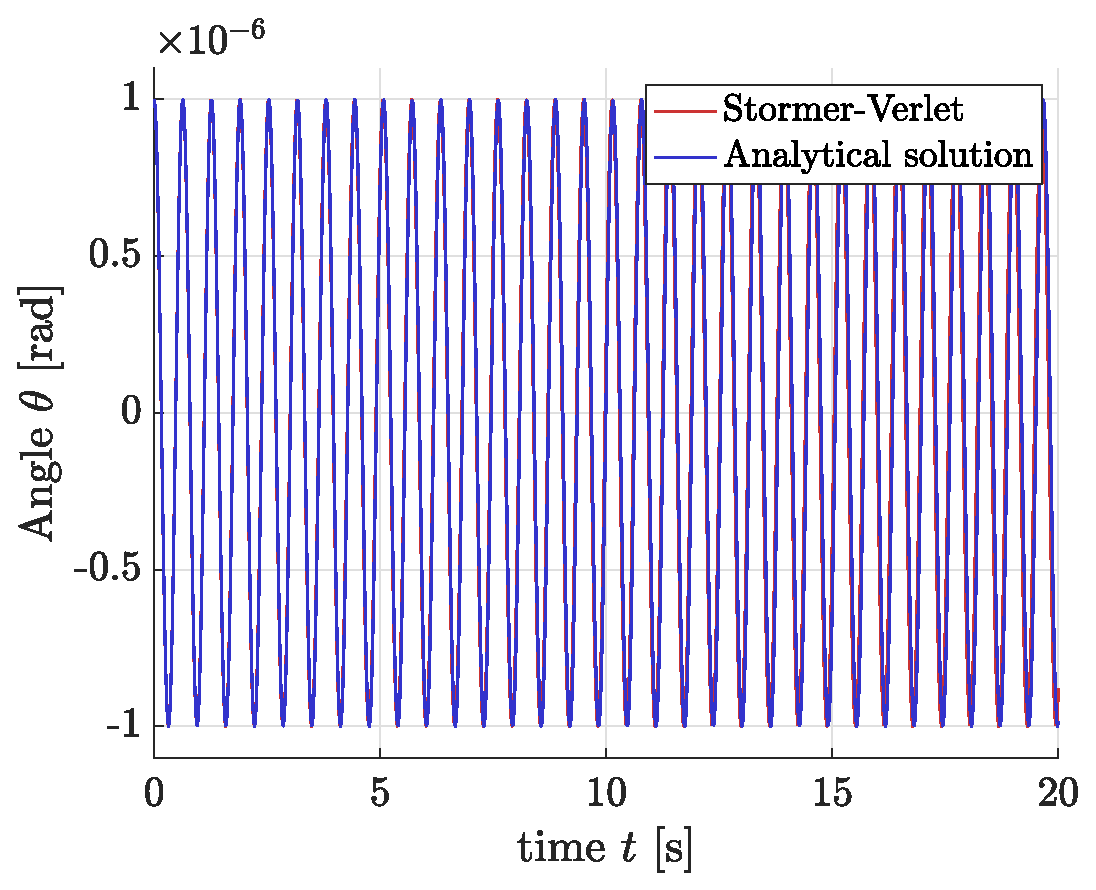
\includegraphics[width=\textwidth]{graphs/a_traj_full.eps}
	\caption{Angle of the pendulum with respect to time, with a comparison between the Stormer-Verlet numerical method and the analytical solution.}
	\label{fig:a-traj-full}
\end{subfigure}
~
\begin{subfigure}[t]{0.48\textwidth}
	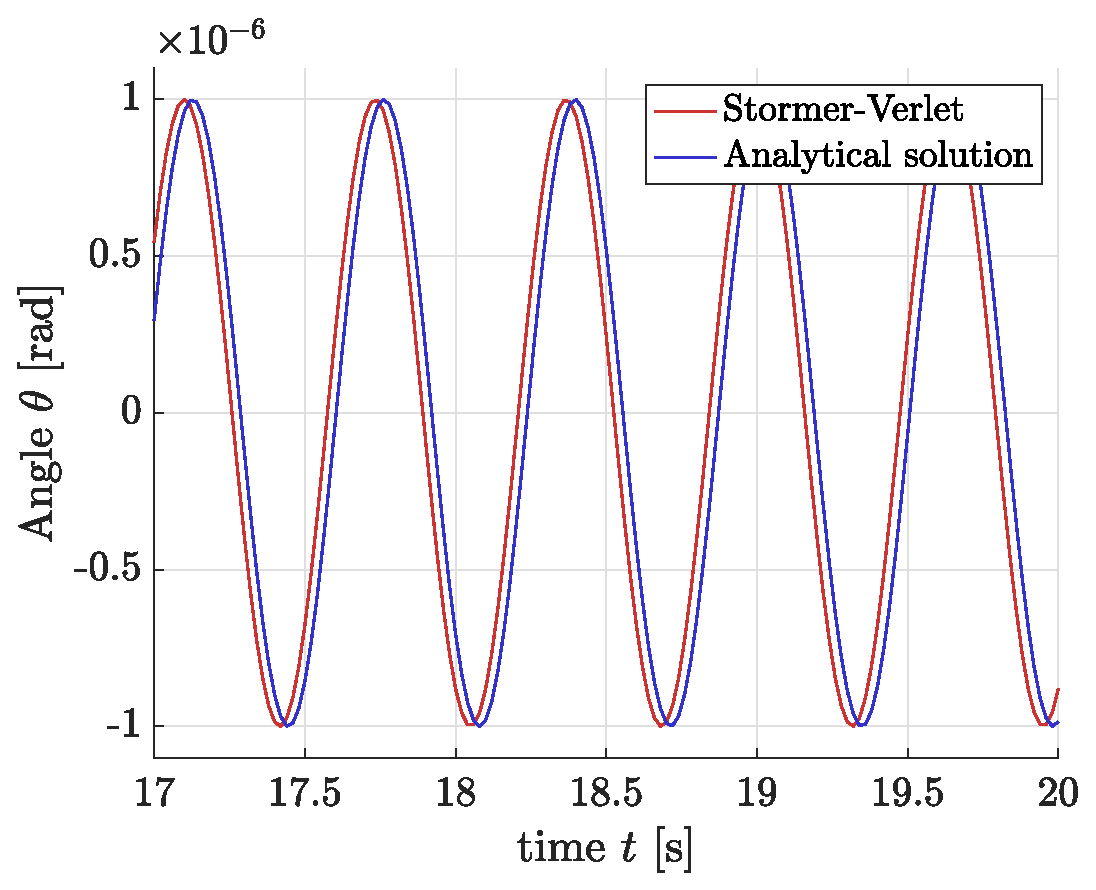
\includegraphics[width=\textwidth]{graphs/a_traj_zoomed.eps}
	\caption{Same plot as \ref{fig:a-traj-full}, with the beginning cropped out to get a better view of the small difference between the numerical and analytical solutions at the end of the simulation.}
	\label{fig:a-traj-zoomed}
\end{subfigure}
\caption{Angle of the pendulum with respect to time, using Stormer-Verlet numerical method at \num{1000} steps and the analytical solution.}
\label{fig:a-traj}
\end{figure}

Figure \ref{fig:a-traj-full} shows a comparison of Stromer-Verlet's numerical method and the analytical solution.
Those plots almost overlap, and the numerical method seems quite accurate knowing the small number of steps considered.
The numerical method seems to be stable over time.
Figure \ref{fig:a-traj-zoomed} shows the same comparison, but focuses on the end of the simulation, where the peak difference occurs.
This slight difference does not seem to affect the amplitude of the sinus, but only its period.
The numerical method has a slightly decreasing period over time.
This comes from computational errors and not from the numerical method, as Stormer-Verlet seems to be stable in this problem.
These errors are probably generated when numbers are rounded.%TODO : Les 2-3 dernières phrases me semblent assez moche, faudrait les modifier.


\subsubsection{Convergence study}
In this section, the convergence of the numerical method of Stormer-Verlet will be studied.

\begin{figure}[h]
\centering
	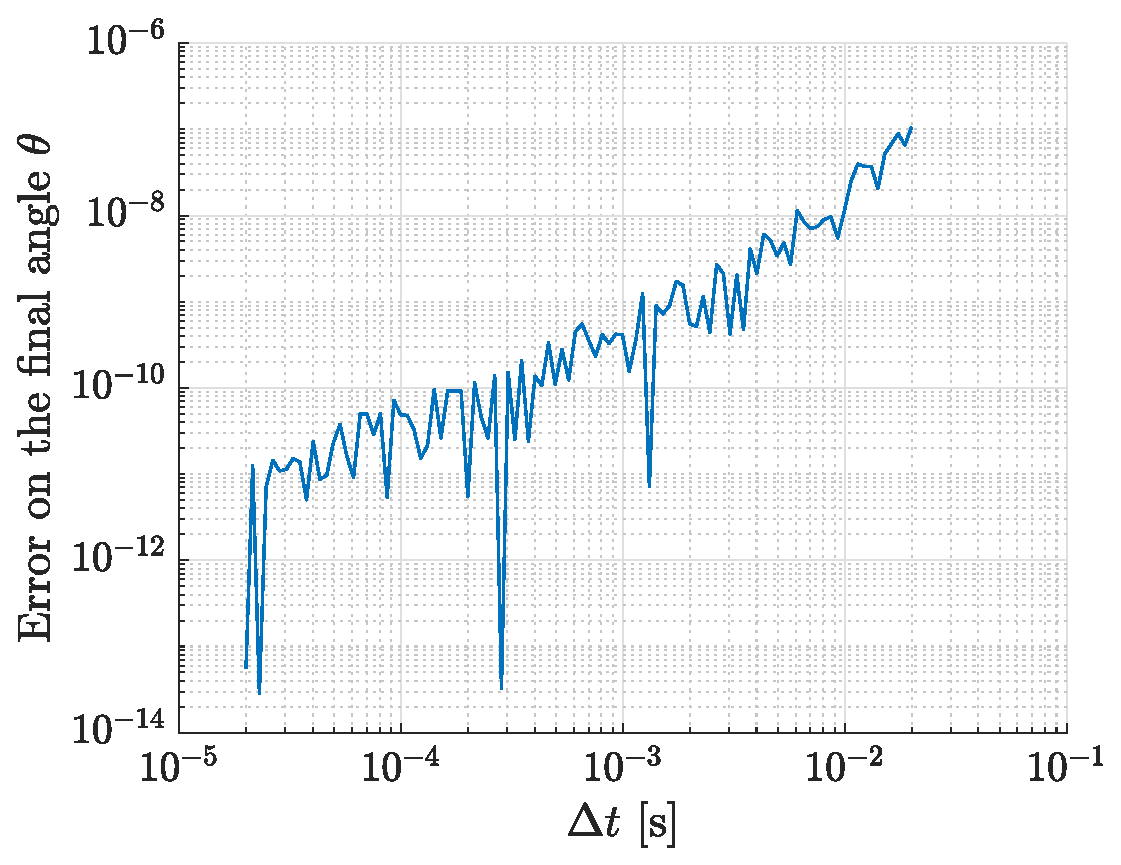
\includegraphics[width=0.6\textwidth]{graphs/a_conv.eps}
	\caption{Error on the final angle of the pendulum with respect to the time step.}
	\label{fig:a-conv}
\end{figure}
%TODO : Il faut refaire cette section
% Ce que je veux dire: L'erreur est divisée par 100 quand le time step est divisé par 10, le fait que le résultat converge parce que ça descend linéairement sur le graph (log), et parler de l'ordre de grandeur de l'erreur.

%Figure \ref{fig:a-conv} shows the convergence study of this problem.
%The first point to verify is the convergence order of the numerical method.
%In this figure, the curve follows an almost constant linear decrease (with a log scale).
%On this plot, dividing the time step by \num{10} almost divides the error by \num{100}.
%This implies a second order numerical method: when the time step is divided by any number $h$, the error is divided by $h^2$.
%For example, at $\Delta t = \SI{d-2}{\second}$ the error is estimated by $err = \num{d-8}$.
%By dividing by \num{10} the time step ($\Delta t = \SI{d-3}{\second}$), the error is now estimated by $err \approx \num{d-10}$, which is \num{100} times smaller.\par
%The second point how small the error gets.
%Consider that the final angle is of order \num{d-6} (fig. \ref{fig:a-traj-full}).
%When the time step is big, $\Delta t = \SI{d-2}{\second}$ for example, the error reaches \SI{10}{\percent}.
%Computations are quite fast and easy to do at this time step.
%Just by lowering a little the time step, the error easily gets smaller that \SI{1}{\percent} or even less, which is gives a good approximation of the problem.
%In summary, Stormer-Verlet's numerical method converges fast, and is fits well the problem in term of convergence.


\subsubsection{Conservation of energy}

\begin{figure}[h]
\centering
	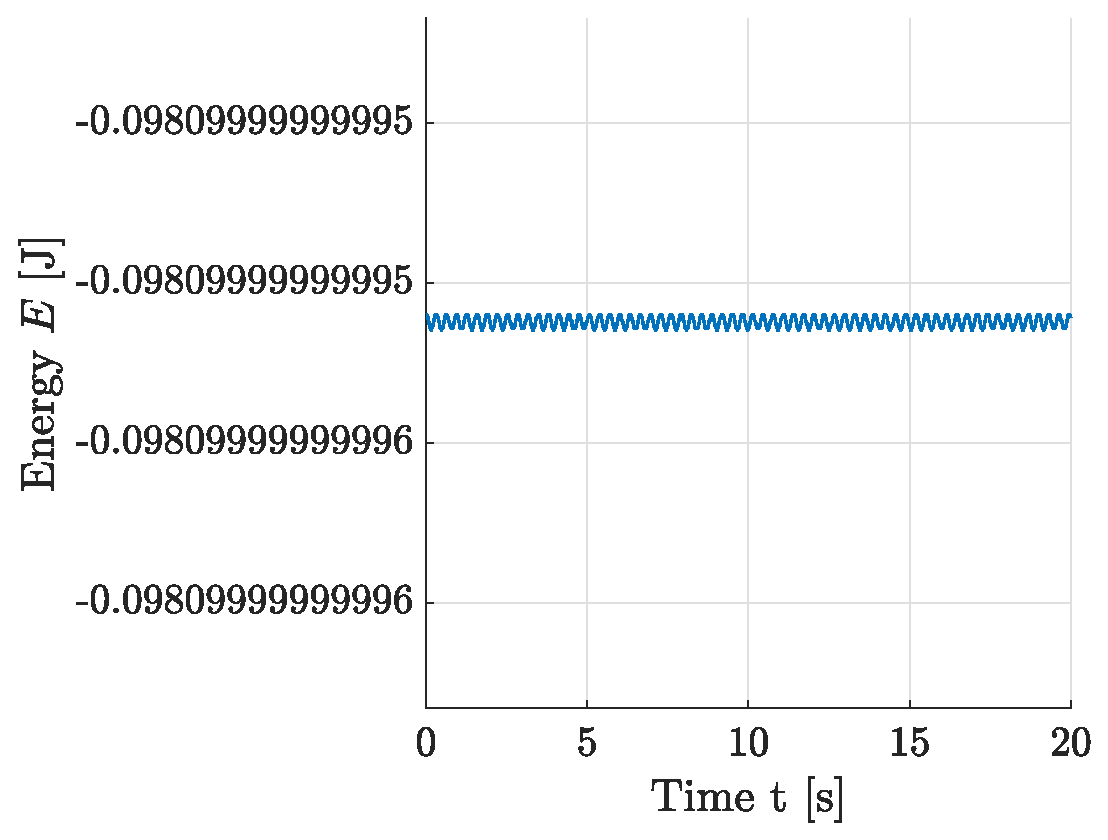
\includegraphics[width=0.6\textwidth]{graphs/a_ener.eps}
	\caption{Study of the mechanical energy of the pendulum with respect to time.}
	\label{fig:a-ener}
\end{figure}

%Ce que je veux dire: L'énergie n'est pas conservée à cause des oscillations, le fait que la variation est très petite sur un nombre pas si petit,  que l'énergie est conservée en moyenne car c'est un schéma symplectique.
Figure \ref{fig:a-ener} shows a study of the mechanical energy over time.
The first information to notice is that mechanical energy does not seem to be conserved even though it should be.
Energy does little oscillation around a point, but does not follow a linear curve.
However, these variations are really small compared to the energy.
The order of magnitude of the energy is \SI{100}{\milli\joule}, where the order of magnitude of the variation of energy is \SI{100}{\pico\joule}. %TODO : Vérifier que ce soit juste. (c'est assez difficile à voir à l'oeil nu)
The variation is so small that it could be easily ignored, and the energy is considered as conserved.
Furthermore, Stormer-Verlet is a symplectic numerical method, which is shown in this figure.
The energy does not grow over time, it is bounded.
The mean mechanical energy is then conserved over time, which implies that, even if the energy is not fully conserved, the numerical method could still be used, as the error would not explode. %TODO : Remplacer 'explode'


\subsection{Great movements: period with respect to amplitude}

\begin{figure}[h]
\begin{subfigure}[t]{0.52\textwidth}
	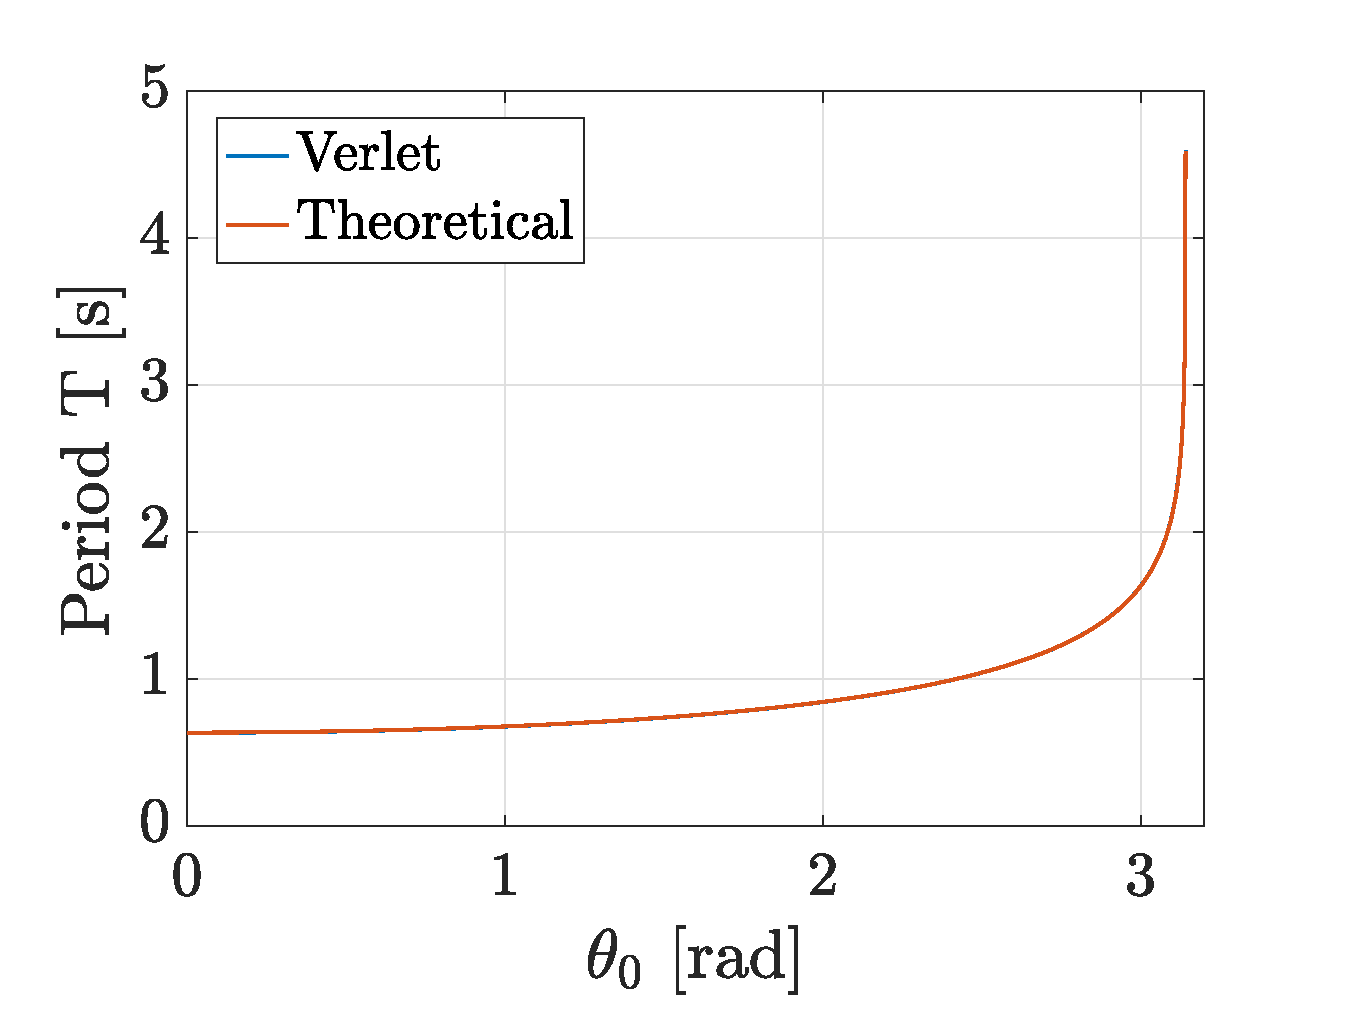
\includegraphics[width=\textwidth]{graphs/b_period.eps}
\end{subfigure}
~
\begin{subfigure}[t]{0.52\textwidth}
	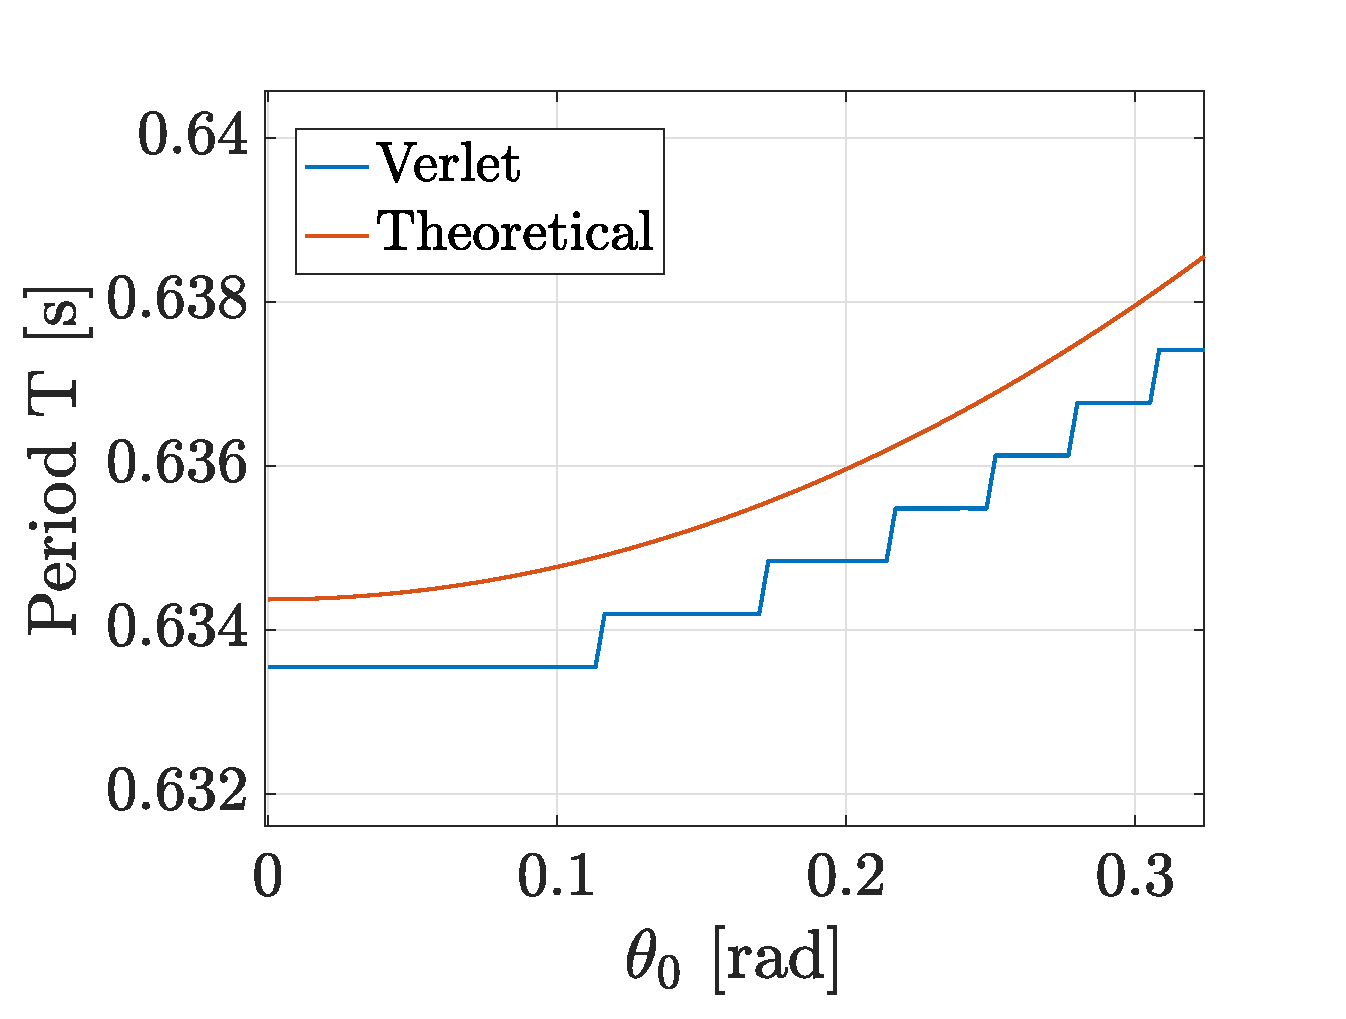
\includegraphics[width=\textwidth]{graphs/b_period_zoom.eps}
\end{subfigure}
\caption{Period of the pendulum with the amplitude $\theta_0 \in ]0,\pi[$ (zoomed in on the right-hand side graph)}
\label{fig:b-period}
\end{figure}

The period of the pendulum was measured over $1000$ simulations with $\theta_0 \in ]0,\pi[$, using the Verlet method, and the resulting plot is shown on figure \ref{fig:b-period}, compared to the analytical solution. As expected, the period grows exponentially with respect to the amplitude.

The difference between the simulation and the theoretical solution is only visible on the zoomed graph, wherein we see that it is of order $10^{-4}$ at this point of the graph. Only part of the graph is shown on the zoomed-in figure, but the two lines stay no less close all throughout and sometimes cross over each other. It is apparent however that the plot showing the Verlet simulations' periods is not as smooth as the theoretical line, as it has a stair-like shape. Overall this comparison shows that the Verlet method has a good precision.

%%%%%%%%%%%%%%%%%%%%%%%%%%%%%%%%%

\subsection{Resonant excitation}
\subsubsection{Verification of the mechanical energy theorem}

The mechanical energy theorem can be written as:
\begin{equation}
	\frac{dE_{mec}}{dt} = P_{nc}
\end{equation}
where $P_{nc}$ is the power of non-conservative forces.

The mechanical energy of the system is:
\begin{equation}
	E_{mec} = \frac{m L^2}{2} \dot{\theta}^2 - mLg \cos \theta
\end{equation}
which gives us its derivative:
\begin{equation}
	\frac{dE_{mec}}{dt} = \frac{m L^2}{2} \dot{\theta} \ddot{\theta} + mLg \dot{\theta} \sin \theta
\end{equation}

\begin{figure}[h]
	\centering
	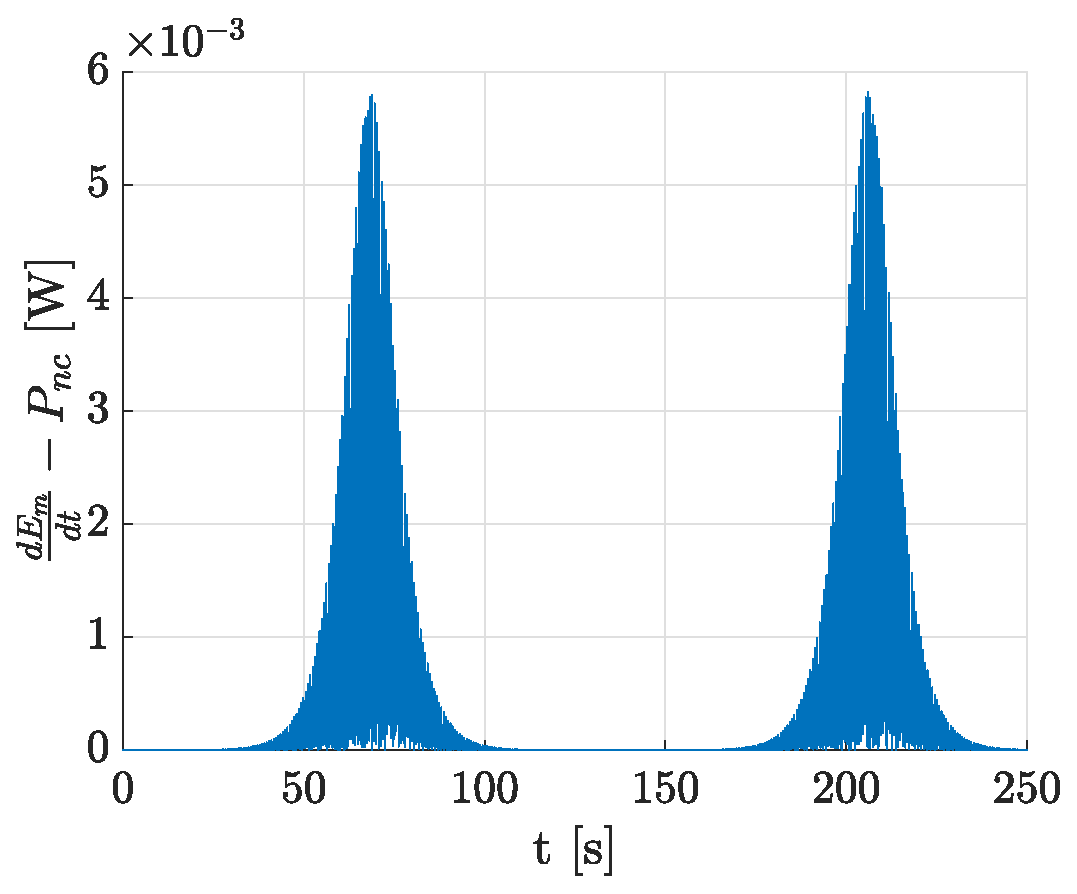
\includegraphics[width=0.6\textwidth]{graphs/c_thm.eps}
	\caption{blabla}
	\label{fig:c-thm}
\end{figure}

\subsubsection{Varying $\Omega$}

%%%%%%%%%%%%%%%%%%%%%%%%%%%%%%%%%

\subsection{Parametric excitation}
\subsubsection{Verification of the mechanical energy theorem}

\begin{figure}[h]
\begin{subfigure}[t]{0.52\textwidth}
	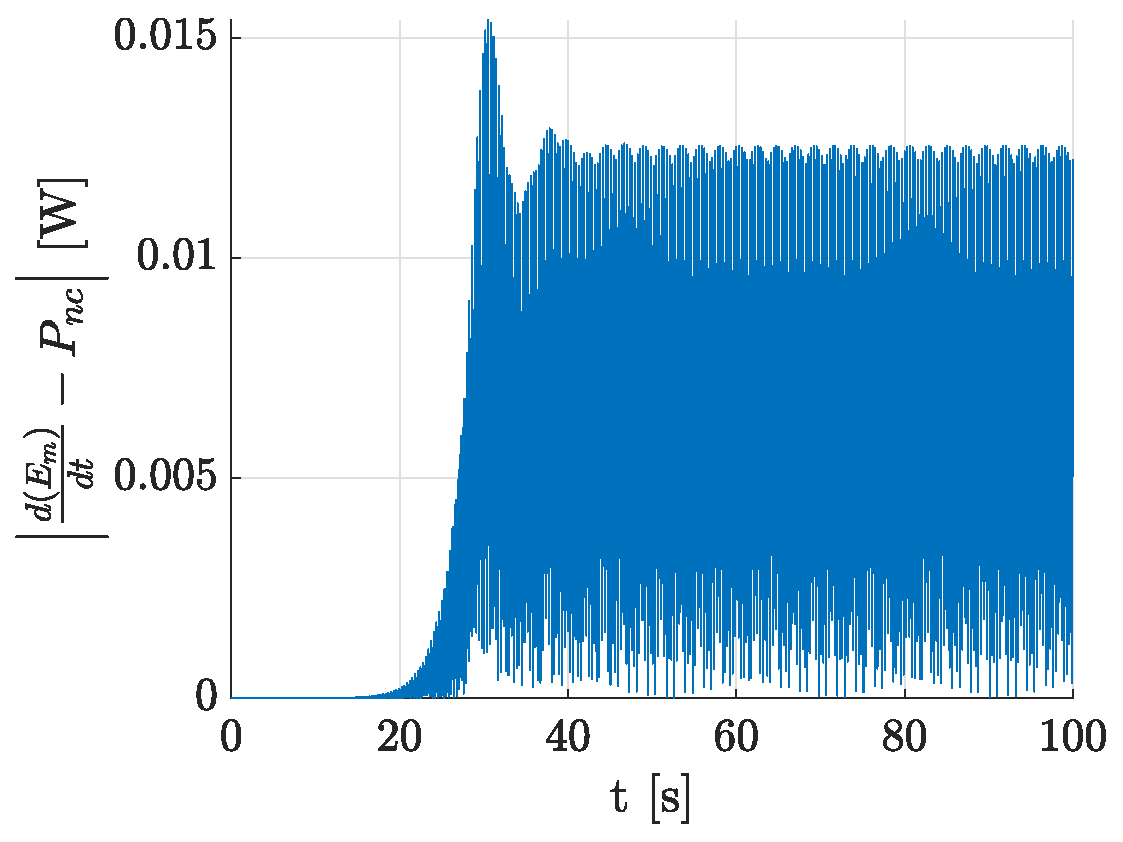
\includegraphics[width=\textwidth]{graphs/d_thm.eps}
\end{subfigure}
~
\begin{subfigure}[t]{0.52\textwidth}
	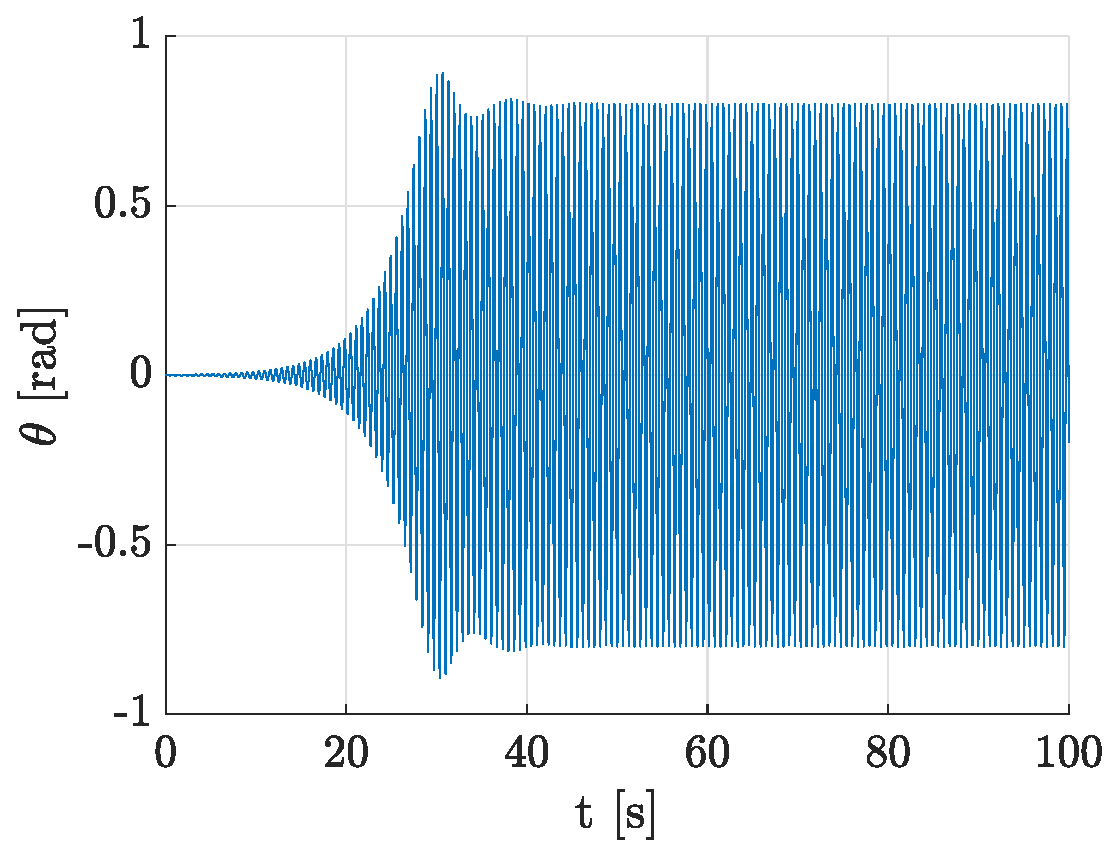
\includegraphics[width=\textwidth]{graphs/d_theta.eps}
\end{subfigure}
\caption{blabla}
\label{fig:d-thm}
\end{figure}

\subsubsection{Varying $\Omega$}

%%%%%%%%%%%%%%%%%%%%%%%%%%%%%%%%%

\subsection{Poincaré section: chaos without air resistance}
\subsubsection{Convergence study on the final angle $\theta$}
\begin{figure}[h]
	\centering
	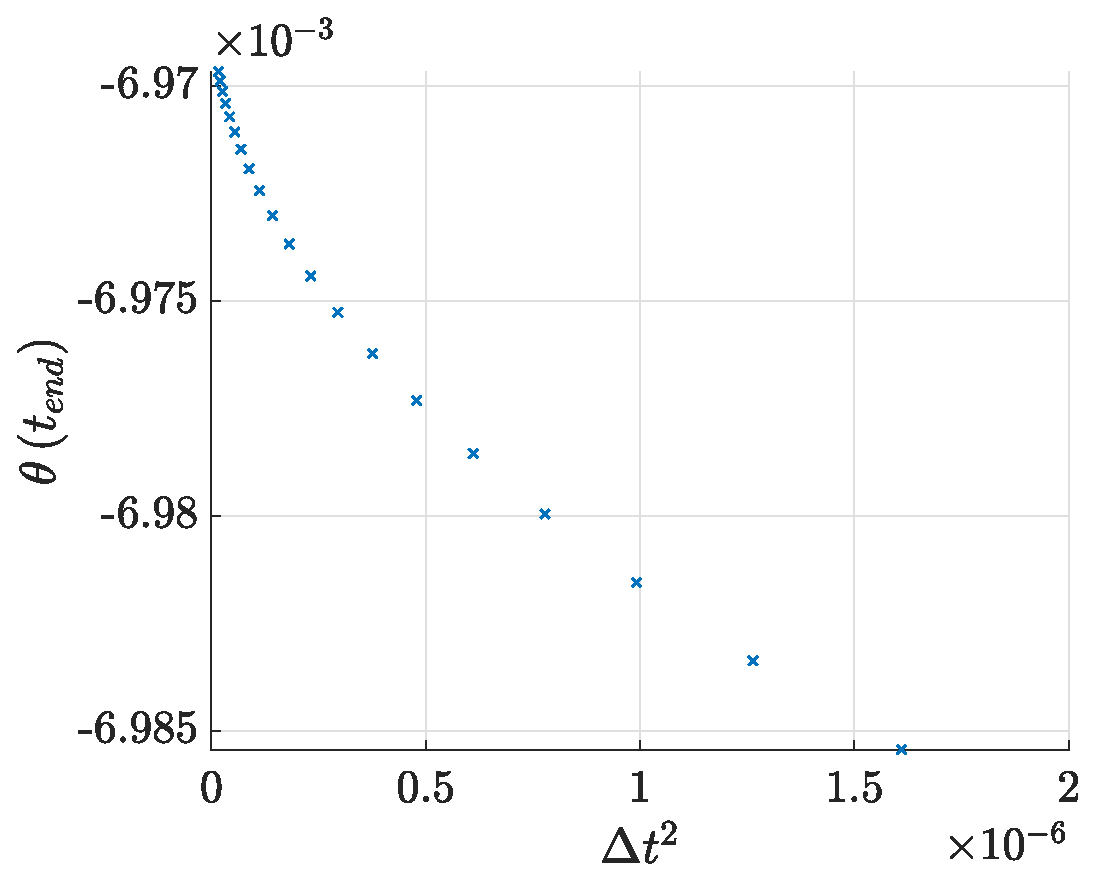
\includegraphics[width=0.6\textwidth]{graphs/e_conv.eps}
	\caption{blabla}
	\label{fig:c-thm}
\end{figure}

\subsubsection{Poincaré sections}
\begin{figure}[h]
	\begin{subfigure}[t]{0.45\textwidth}
		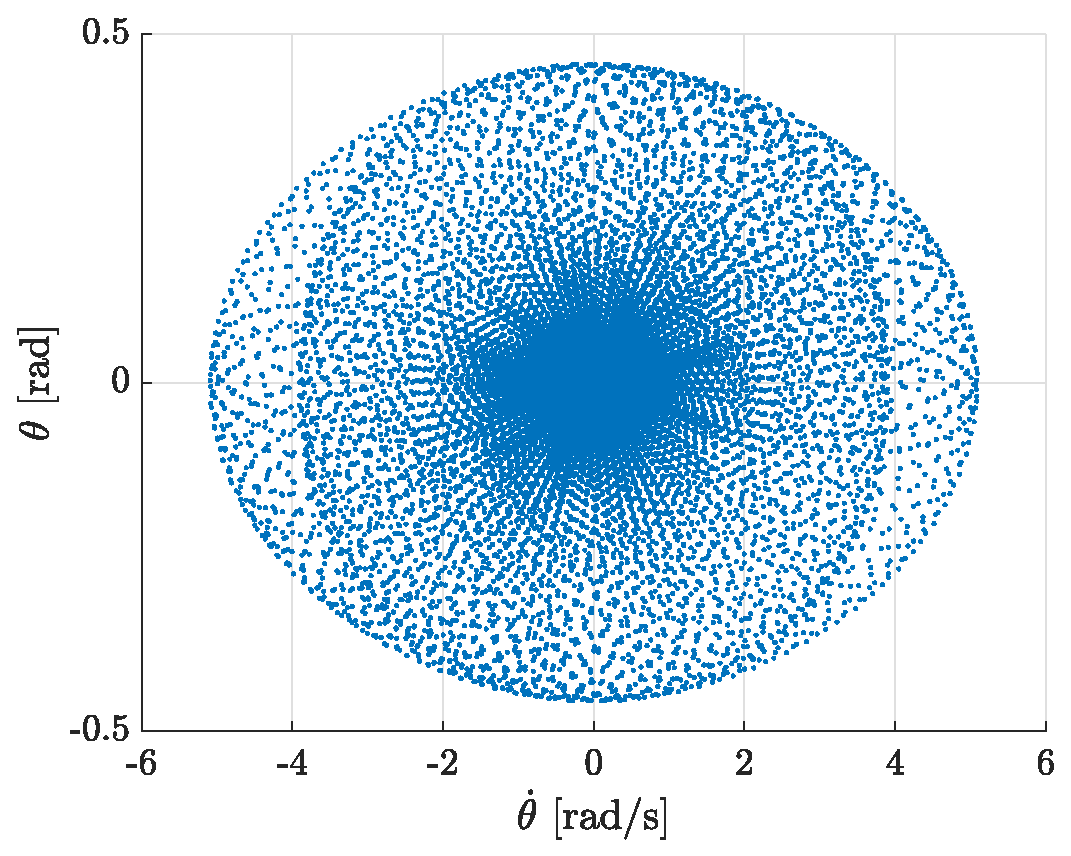
\includegraphics[width=\textwidth]{graphs/e_poincare_bigbrother.eps}
		\caption{blabla}
		\label{fig:e-pc-bigbrother}
	\end{subfigure}
	~
	\begin{subfigure}[t]{0.45\textwidth}
		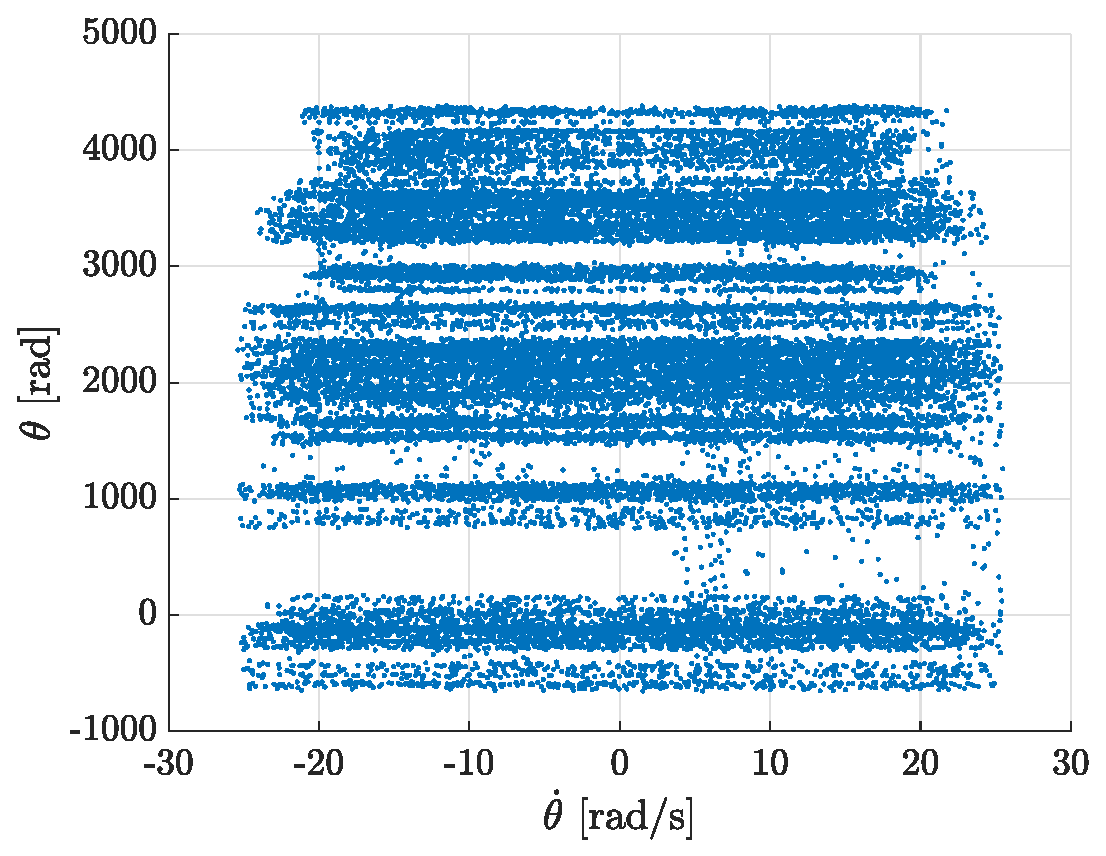
\includegraphics[width=\textwidth]{graphs/e_poincare_chaos.eps}
		\caption{blabla}
		\label{fig:e-pc-chaos}
	\end{subfigure}
	\newline
	\begin{subfigure}[t]{0.45\textwidth}
		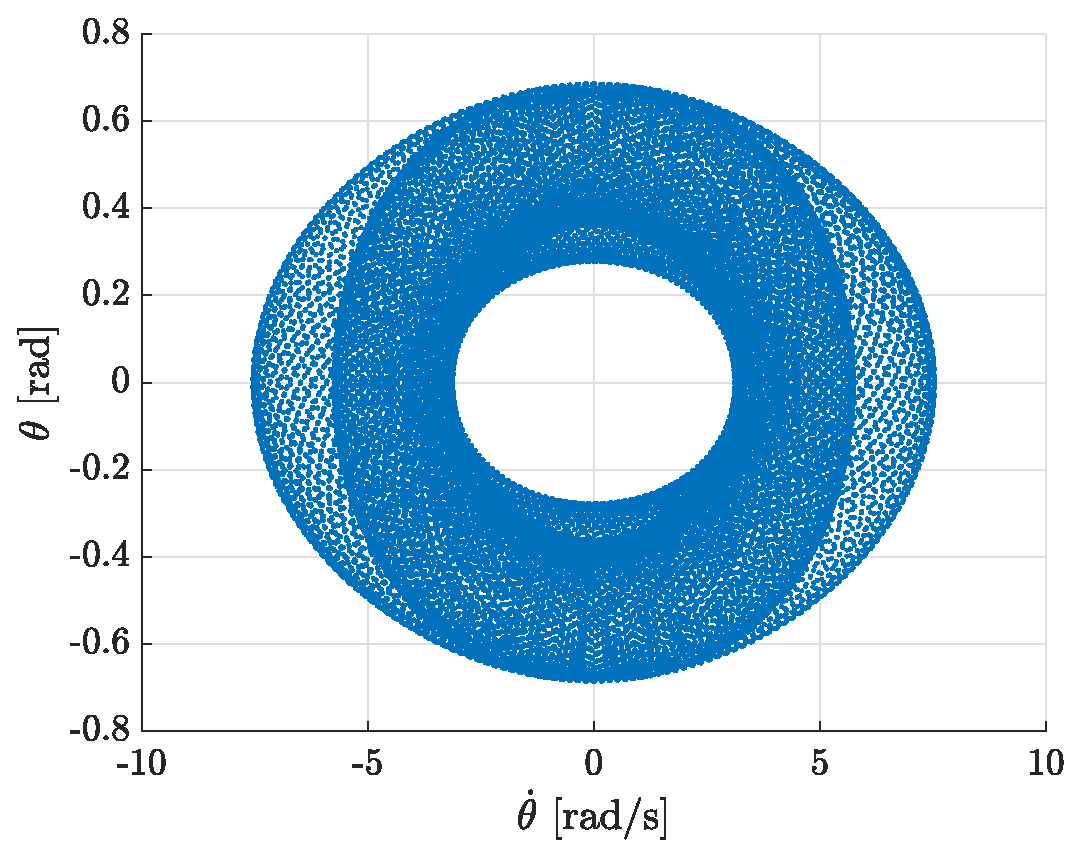
\includegraphics[width=\textwidth]{graphs/e_poincare_fatdonut.eps}
		\caption{blabla}
		\label{fig:e-pc-fatdonut}
	\end{subfigure}
	~
	\begin{subfigure}[t]{0.45\textwidth}
		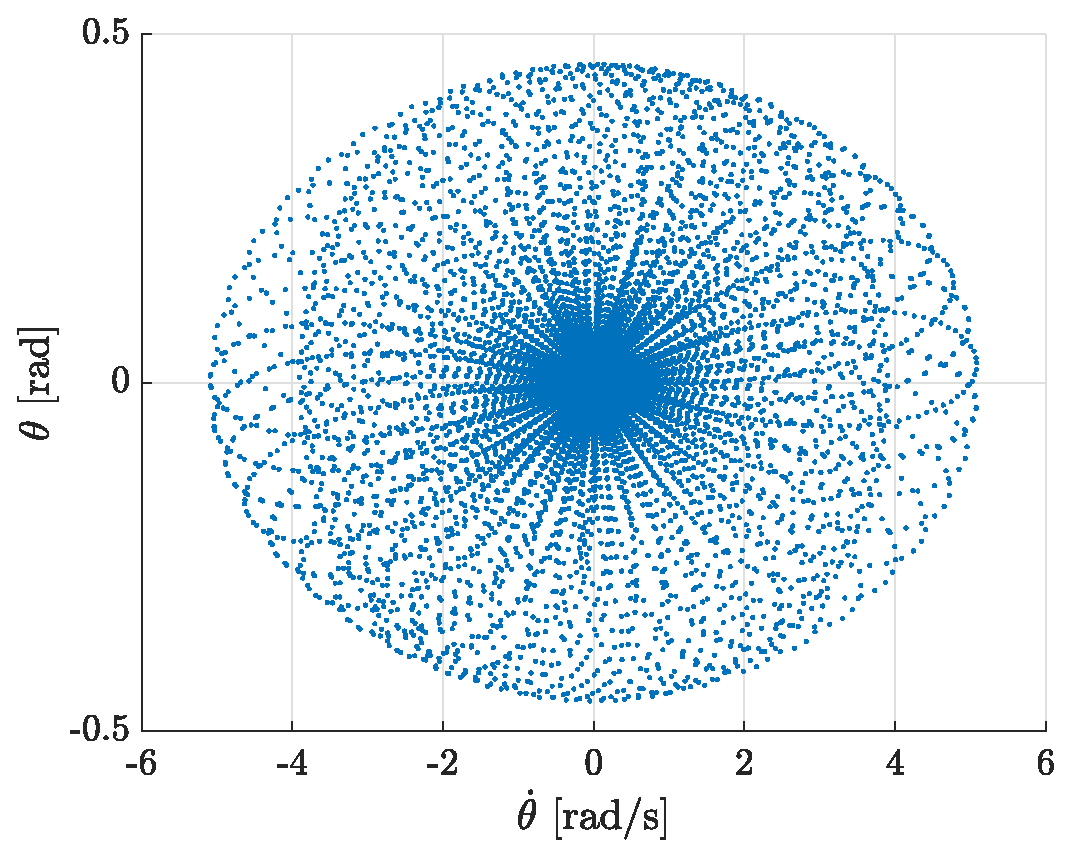
\includegraphics[width=\textwidth]{graphs/e_poincare_littlemoves.eps}
		\caption{blabla}
		\label{fig:e-pc-littlemoves}
	\end{subfigure}
	\caption{blabla}
	\label{fig:e-pc}
\end{figure}

%%%%%%%%%%%%%%%%%%%%%%%%%%%%%%%%%

\subsection{Pointcaré section: chaos with air resistance}

\end{document}
